\chapter{Introduction to Gravitational Lensing}

One of the most interesting consequences of Einstein's theory of general relativity, regarding the distortion of space time by massive objects is gravitational lensing. The basic principle behind gravitational lensing is that light is distorted when it travels close to the potential well (the distortion of space time) of massive objects which is an analogous effect to the one caused by optical lenses. 

Although the discovery of gravitational lensing was made only in the past century, the possibility that there could be such a deflection had been suspected much earlier, by Newton and Laplace among others (Narayan, Ramesh et. al. \citeyear{Reference25}). Johann Gerog von Soldner in 1801 calculated the magnitude of the deflection due to the Sun, assuming that light consists of material particles and using Newtonian gravity. Later, Einstein (1911) employed the equivalence principle to calculate the deflection angle and re-derived Soldner’s formula. Later yet, in 1915 Einstein applied the full field equations of General Relativity and discovered that the deflection angle is actually twice his previous result, the factor of two arising because of the curvature of the metric. According to this formula, a light ray which tangentially grazes the surface of the Sun is deflected by 1.7''. Einstein’s final result was confirmed in 1919 when the apparent angular shift of stars close to the limb of the Sun (see Fig. [1]) was measured during a total solar eclipse (Dyson, Eddington, \& Davidson 1920). The quantitative agreement between the measured shift and Einstein’s prediction was immediately perceived as compelling evidence in support of the theory of General Relativity.

Gravitational lensing can be separated into two main categories which are its two most important ways to manifest.

\textbf{1. Strong lensing:} Where there are easily visible distortions such as the formation of Einstein rings, arcs, and multiple images.

\textbf{2. Weak lensing:} Where the distortions of background sources are much smaller and can only be detected by analysing large numbers of sources in a statistical way to find coherent distortions of only a few percent.

\begin{figure}[H]
\centering
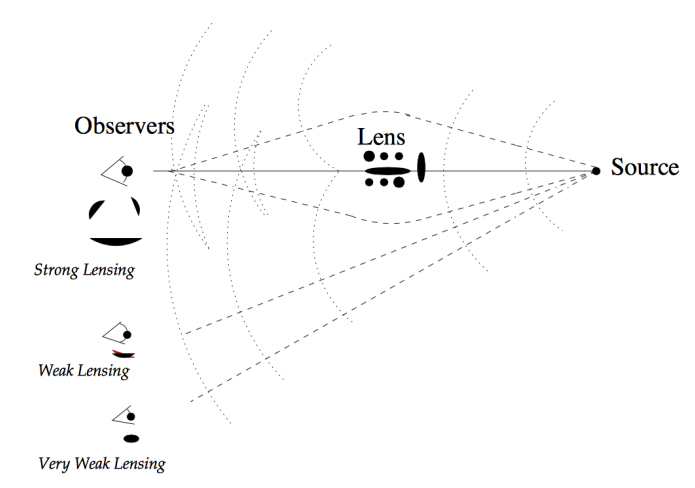
\includegraphics[width=12cm]{images/types_of_lensing.png}
\caption[Types of lensing]{Types of lensing. Courbin, F. et al \citeyear{Reference24}}
\end{figure}

Figure [2.1] sketches the effects of gravitational lensing in the strong, weak and very weak lensing regimes. As seen in the figure, under certain conditions the background source can be seen in multiple images and ``arcs" surrounding the lensing object, which is the strong lensing regime and will be the useful regime for this work. 

\section{Gravitational Lensing formalism}

For the generalities of gravitational lensing we follow the order given in a review by Massimo Meneghetti (\citeyear{Reference26}) in which we first start by introducing the deflection angle which is the measure of the angular distance that has been deflected and which is linearly dependent on the mass $\text{M}$. This dependence ensures that the angles of deflection of an array of lenses can be superposed linearly. If we had N point masses sparsed on a plane, with positions $\xi_i$ and masses $\text{M}_{i}$, then the deflection angle would be:

\begin{equation}
\hat{\vec{\alpha}}(\vec{\xi})=\sum_{i}\hat{\vec{\alpha_{i}}}(\vec{\xi}-\vec{\xi_{i}})=\frac{4G}{c^{2}}\sum_{i}M_{i}\frac{\vec{\xi}-\vec{\xi_{i}}}{\left|\vec{\xi}-\vec{\xi_{i}}\right|^{2}}
\end{equation}

Fortunately, in most three dimensional distributions of matter (even in the case of lensing by massive objects like galaxy clusters) the physical size of the lens is generally much smaller than the distances between the observer, the lens and the source. This means that the deflection of light takes place in a very thin and short section of its path to the observer. Given this, we can use the \textit{thin screen approximation}: ``The lens is approximated by a planar distribution of matter, the lens plane". Also the sources can be treated as if they lie on a plane which is called the source plane.

The \textit{thin screen approximation} alows us to state that the lensing matter distribution is fully described by its surface density

\begin{equation}
\Sigma(\vec{\xi}) = \int \rho (\vec{\xi},z)dz
\end{equation}

where $\vec{\xi}$ is a two-dimensional vector on the lens plane and $\rho$ is the three dimensional density.

\begin{figure}[H]
\centering
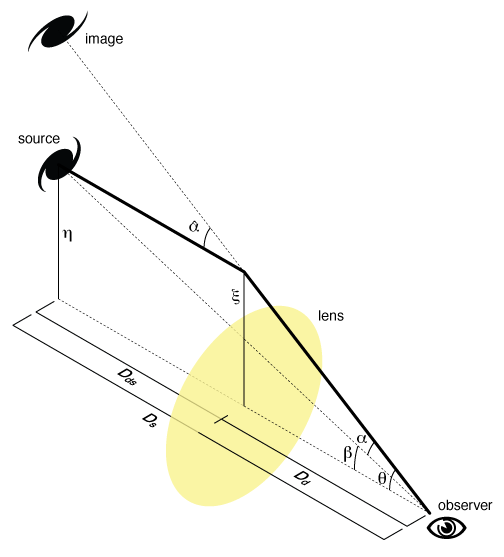
\includegraphics[width=11cm]{images/lensing.png}
\caption[Angles in gravitational lensing]{Sketch of a lensing configuration, where $D_{ds}$ is the distance from the lense to the source, $D_s$ is the distance from the observer to the source and $D_d$ is the distance from the observer to the source. Image by Michael Sachs, Wikipedia}
\end{figure}

Figure [2.2] is a sketch of a typical gravitational system. The lensing mass is located at a angular diameter distance $D_d$ and it deflects the light rays coming from a source at an angular distance of $D_s$.

The optical axis is perpendicular to the lens and source planes and passes through the observer. We measure the angular positions on both planes with respect to this reference direction. The source is at the angular position $\vec{\beta}$ and lies on the source plane at a distance $\vec{\eta}=\vec{\beta}D_s$ from the optical axis. The deflection angle $\hat{\vec{\alpha}}$ of the light ray comes from the source and has impact parameter $\vec{\xi}=\vec{\theta}D_d$ on the lens plane. Due to this deflection, the observer receives the light coming from the source as if it was emitted at the angular position $\vec{\theta}$.

If $\vec{\theta}$, $\vec{\beta}$ and $\hat{\vec{\alpha}}$ are small, the true position of the source and its observed position on the sky are related by a very simple relation, obtained by a geometrical construction. This relation is called the lens equation and is written as

\begin{equation}
\vec{\theta}D_s = \vec{\beta}D_s+ \hat{\vec{\alpha}}D_{ds}     \\\\\\\\\\\
\end{equation}

where as seen in the figure, $D_{ds}$ is the distance between the lens and the source.

Defining the reduced deflection angle

\begin{equation}
\vec{\alpha}(\vec{\theta})\equiv \frac{D_{ds}}{D_s}\hat{\vec{\alpha}}(\vec{\theta})
\end{equation}

And from equation 2.3 we get

\begin{equation}
\vec{\beta}=\vec{\theta}-\vec{\alpha}(\vec{\theta})
\end{equation}

The most interesting physics of the simple lens equation arises because $\vec{\alpha}$ depends on $\vec{\theta}$. Now, we can characterize an extend the distribution of matter by its effective lensing potential, which is obtained by projecting the three-dimensional Newtonian potential on the lens plane and scaling it accordingly

\begin{equation}
\hat{\Psi}(\vec{\theta})=\frac{D_{ds}}{D_{d}D_{s}}\frac{2}{c^{2}}\int\Phi(D_{d}\vec{\theta},z)dz
\end{equation}

This lensing potential satisfies two important properties:

1) The gradient of $\Psi$ gives the scaled deflection angle:

\begin{equation}
\vec{\nabla}_{x}\Psi(\vec{x})=\vec{\alpha}(\vec{x})
\end{equation}

2) The Laplacian of $\Psi$ gives twice the convergence

\begin{equation}
\Delta_{x}\Psi(\vec{x})=2\kappa(\vec{x})
\end{equation}

where the convergence is defined as a dimensionless surface density

\begin{equation}
\kappa(\vec{x})\equiv \frac{\Sigma(\vec{x})}{\Sigma_{cr}}\qquad \text{with} \qquad \Sigma_{cr}=\frac{c^{2}}{4\pi G}\frac{D_s}{D_d D_{ds}}
\end{equation}

$\Sigma_{cr}$ is called the critical surface density and it characterizes the lens system and which is a function of the angular diameter distances of lens and source. Now let's introduce the distortion.

One of the main features of gravitational lensing is that it distorts the shapes of the sources, this is particularly evident when the source has no negligible apparent size. In some cases the background galaxies can appear as very long arcs in galaxy clusters as mentioned at the beginning of this chapter. 

The effect of distortion takes place because light bundles are deflected differentially. In the ideal case, the shape of the background images can be determined by solving the lens equation for all the points within the extended source. In particular, if the source is much smaller than the angular size on which the physical properties of the lens change, the relation between the source and image positions can locally be linearised. Mathematically this means that the distortion of images can be described by the Jacobian matrix

\begin{equation}
A\equiv\frac{\partial\vec{y}}{\partial\vec{x}}=\left(\delta_{ij}-\frac{\partial\alpha_{i}(\vec{x})}{\partial x_{j}}\right)=\left(\delta_{ij}-\frac{\partial^{2}\Psi(\vec{x})}{\partial x_{i}\partial x_{j}}\right)
\end{equation}

where $x_i$ indicates the $i$-component of $\vec{x}$ on the lens plane. It shows that the elements of the Jacobian matrix can be written as combinations of the second derivatives of the lensing potential. It is useful to use the shorthand notation

\begin{equation}
\frac{\partial^{2}\Psi(\vec{x})}{\partial x_{i}\partial x_{j}}\equiv\Psi_{ij}
\end{equation}

Let's split off an isotropic part from the Jacobian:

\begin{equation}
\left(A-\frac{1}{2}\text{tr}A\cdot I\right)_{ij}=\left(\begin{array}{cc}
-\frac{1}{2}\left(\Psi_{11}-\Psi_{22}\right) & -\Psi_{12}\\
-\Psi_{12} & \frac{1}{2}\left(\Psi_{11}-\Psi_{22}\right)
\end{array}\right)
\end{equation}

this is the shear matrix, which is an antisymmetric, trace-free matrix that quantifies the projection of the gravitational tidal field (the gradient of the gravitational force), which describes distortions of background sources.  This allows us to define the pseudo-vector $\vec{\gamma}=(\gamma_1 , \gamma_2)$ on the lens plane, whose components are

\begin{equation}
\gamma_1(\vec{x})=\frac{1}{2}(\Psi_{11}-\Psi_{22})\qquad \text{and} \qquad \gamma_2(\vec{x})=\Psi_{12} = \Psi_{21}
\end{equation}

This is called the shear. The eigenvalues of the shear matrix are 

\begin{equation}
\pm \sqrt{\gamma_1^2 + \gamma_2^2} = \pm \gamma
\end{equation}

Thus, there exists a coordinate rotation by an angle $\phi$ such that 

\begin{equation}
\left(\begin{array}{cc}
\gamma_{1} & \gamma_{2}\\
\gamma_{2} & -\gamma_{1}
\end{array}\right)=\gamma\left(\begin{array}{cc}
\cos2\phi & \sin2\phi\\
\sin2\phi & -\cos2\phi
\end{array}\right)
\end{equation}

And for the trace we have

\begin{equation}
\frac{1}{2}\text{tr}A=(1-\kappa)\delta_{ij}
\end{equation}

Thus the Jacobian becomes 

\begin{equation}
A= \left(\begin{array}{cc}
1-\kappa-\gamma_{1} & -\gamma_{2}\\
-\gamma_{2} & 1-\kappa+\gamma_{1}
\end{array}\right)
\end{equation}

Where $\kappa$ is the convergence that determines the magnification and $\gamma_{1}$ and $\gamma_{2}$ are the shear components that determine the distortion of the background objects. More precisely, the convergence describes the isotropic focusing of light rays while the shear describes the effect of tidal gravitational forces. Convergence acting alone leads to an isotropic magnification or demagnification while the shear induces distortions in the shapes of lensed images (Wright \& Brainerd, \citeyear{Reference4}). 

Finally, we can introduce another useful quantity in the characterization of gravitational lensing systems. The \textit{magnification} is quantified by the inverse of the determinant of the Jacobian matrix. For this reason, the matrix $\text{M}=A^{-1}$ is called the \textit{magnification tensor}, and we define

\begin{equation}
\mu \equiv \text{det} M = \frac{1}{\text{det}A}=\frac{1}{(1-\kappa)^2-\gamma^2}
\end{equation}

The eigenvalues of the magnification tensor measure the amplification in the tangential and in the radial direction and are given by

\begin{equation}
\mu_t = \frac{1}{\lambda_t}=\frac{1}{1-\kappa - \gamma} \qquad \text{and} \qquad  \mu_r = \frac{1}{\lambda_r}=\frac{1}{1-\kappa + \gamma}
\end{equation}

The magnification is ideally infinite where $\lambda_t=0$ and where $\lambda_r=0$. These two conditions define two curves in the lens plane, called the tangential and the radial critical line, respectively. An image forming along the tangential critical line is strongly distorted tangentially to this line. On the other hand, an image forming close to the radial critical line is stretched in the direction perpendicular to the line itself. 

In the inner region of galaxy clusters we are in the strong lensing regime so we will focus our discussion on strong lensing and the search for multiple images and arcs in the inner regions of the galaxy clusters. Figure [2.3] is a representation of a lensing system in which a background galaxy is lensed by a cluster of galaxies and produces multiple images and arcs observed by our telescopes. 

\begin{figure}[H]
\centering
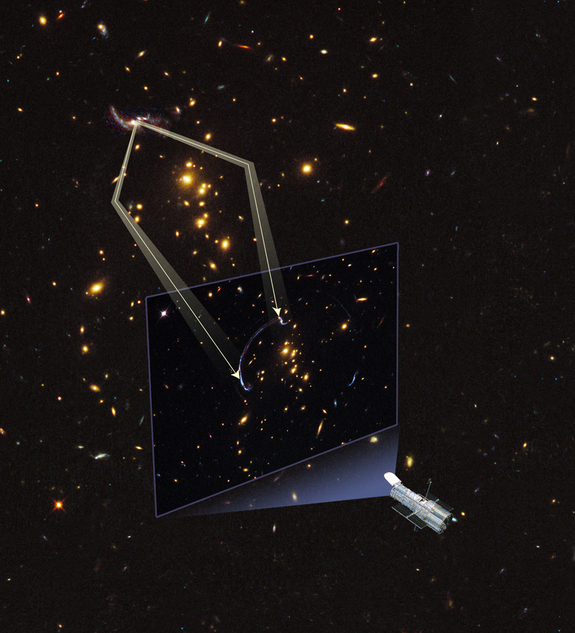
\includegraphics[width=12cm]{images/lensing.jpg}
\caption[Strong Lensing representation]{Representation of strong lensing by a galaxy cluster. Credits to Nasa}
\end{figure}

Now, let's understand in what scales we can use gravitational lensing to study these massive systems.